\section{Considerações iniciais}

Segundo o relatório técnico \citeonline{MineralCommodity2007} o concreto é atualmente considerado o material estrutural mais utilizado no mundo, e ficando em segundo lugar em materiais gerais perdendo apenas para a água. 
Os cálculos apresentados por \citeonline{Gagg2014} relatam que há o dobro de concreto sendo utilizado em construções do que há somando a utilização de aço, alumínio, madeira e plástico, com isso podendo ser encontrados na maioria das categorias de construções, desde casas de alvenaria até pontes, usinas e plataformas de extração petrolíferas \cite{Lima2014}.

Nessa linha de raciocino, é necessário entender o básico de seus conceitos e sua contextualização na problemática desta pesquisa, logo, nesse capítulo serão abordados os conceitos de concreto, sua aplicação em OAE`s, suas variações de aplicações, o limite de sua vida útil e patologias.

\section{Conceitos gerais}

Embora seja um material muito conhecido, ainda há uma falta de entendimento principalmente pelos cidadães comuns, que podem não saber diferencial concreto de cimento já que ambos termos serem comumente usados de forma conjunta \cite{Gagg2014}, 
isso acontece por conta que o concreto é uma massa resultante da mistura de diversas materiais, sendo o principal destes o cimento, que é o material aglutinante deste compósito, agrupando todos os materiais que compõem o concreto. \cite{allen2019fundamentals}.

Essa mistura pode ser modificada, porém a receita padrão é a mistura de água, cimento, agregados miúdos como areia, e agregados graúdo como cascalho, aditivos e adições; dependendo da porcentagem presente de cada ingrediente diferentes características poderão aparecer no concreto, além de impactar sua resistência, que é a quantidade de força de compressão resistida pelo concreto, sendo geralmente medido em \sigla{MPa}{Megapascal} \cite{pinheiro2007fundamentos}. 
Tais diferenças de medidas são desejáveis e que permitem o concreto ser utilizado mundialmente já que cada lugar há diferentes necessidades, locais com muita umidade, muito sol, chuvas fortes ou construções de grande peso como pontes, para cada um desses há uma receita diferente e geralmente cabe ao engenheiro tecnologista do concreto estipular tais características garantindo assim especificações mínimas conforma as normas de projeto de cada país. \cite{izharcomparison}.

A principal característica do concreto é sua versatilidade que acontece por se tratar de uma mistura que em primeiro momento está em um estado físico líquido, podendo ser moldado de acordo com a necessidade alterando sua forma para se adequar a diferentes tipos de estruturas, como pilares, paredes, piso, entre outros \cite{Gagg2014}. Após um período de espera o concreto se enrijece saindo de seu estado líquido até um estado sólido onde se obtêm uma grande resistência à compressão.


\section{Concreto armado}

O concreto armado é um material que emprega o concreto tradicional e uma adição de barras de aço, onde ambos se complementam para resistir respectivamente às forças de compressão e tração \cite{Lima2014}. 
Essas barras de aço, chamadas de armadura do concreto oferecem ao concreto a resistência necessária para combater esforços de tração, necessária em todas as peças estruturais que formam edificações, pontes e outras estruturas. \cite{pinheiro2010estruturas}.

\section{Obra de arte especial}

De acordo com a definição pelo engenheiro civil e pesquisador \citeonline{Ciro2014}, \sigla{OAE}{Obra de Arte Especial} são construções estruturais com finalidade transpor grandes obstáculos, tais quais como rios, desníveis, porções urbanas, entre outros; dessa forma, se configura como OAE estruturas como pontes quando construídas sobre níveis de água, como viadutos quando sobre avenidas ou espaços secos ou como túneis em casos abaixo da superfície.

No Brasil, o principal órgão regulador dessas estruturas, a nível federal, é o \sigla{DNIT}{Departamento Nacional de Infraestrutura de Transporte} autarquia responsável por implementar a política de infraestrutura de transportes terrestres e aquaviários,
estabelecendo as regras de construção e monitoramento que devem ser seguidas pelos construtores \cite{dnitdados}.

Como dito anteriormente, o concreto, principalmente o concreto armado, possui uma incrível resistência á compressão, fazendo-o uma ótima escolha como elemento principal na construção das OAE's, ainda mais quando comparado seu custo operacional e disponibilidade no mercado \cite{santos2008armaccao}. 
Porém como todo material estrutural o concreto possui uma vida útil que é pré-estabelecida em função do seu tipo de aplicação. O material ao longo dessa vida útil sofre com a ação das forças da natureza e depreciação por uso, perdendo parte desta resistência mecânica \cite{santos2008armaccao}. Portanto estudar meios para planejar reparos na estrutura são técnicas importantes no estudo das estruturas de concreto.

Por conta de tais fatores o DNIT torna obrigatório o monitoramento das OAE's,  habitualmente a cada dois anos, sendo obrigatório a presença de inspetores qualificados com anos de experiência e inspetores auxiliares em um processo demorado da criação de um relatório que envolve a observação de toda a OAE, captura de evidências visuais como fotos ou vídeos e descrição por escrito da situação da OAE, de suas falhas e expectativa para os próximos anos \cite{dnit2004}.

\section{Falhas estruturais}

De acordo com o conceito relatado por \citeonline{afonso2021}, falhas estruturais são quando um componente estrutural ou até mesmo toda a estrutura perde a capacidade de uso determinada em projeto, tais falhas podendo ser classificadas de acordo com seu fator expositivo. 
Em especial para esta pesquisa, as falhas causadas por conta de fraturas são chamadas de falha frágil sendo geralmente resultante de se danos acumulados, que com o tempo fazem com que o material estrutural perca sua resistência, dessa forma também sendo configurado como um dano progressivo \cite{anneLink2016}.

 Segundo \citeonline{cremonini1988incidencia}, o concreto é de fato um material com uma resistência muito alta, tanto em questão de cargas quanto em agressões ambientais, porém essa resistência pode vir a ruir, comprometendo sua capacitância de suportar os empenhos solicitados. 
 Ao fazer o estudo dos causadores dessa perda de resistência, a engenharia emprega o termo patologia aos tipos de causas e origens de tais problemas \cite{cremonini1988incidencia}
 
 Á vista disso, é imprescindível  que se tenha a realização de estudos sobre tais patologias e como evitá-las. Com isso, algumas das patologias mais comuns \cite{statera} encontradas são:

\begin{description}
    \item[Fissuras:]
    A ocorrência de fissuras em estruturas que utilizam concreto armado podem implicar em sérios problemas estruturais e simbolizam sérios problemas de estado de conservação, nos piores casos, com a falta de manutenção apropriada faz com que toda a estrutura se comprometa, perdendo todo seu caráter estético, social econômico ademas dos riscos de segurança ao usuário \cite{santos2014patologia}.
    
    Dessa forma, é fato que fissura é um problema de enorme importância que abrange diversas áreas, desde econômicas até da satisfação psicológica dos usuários da estrutura \cite{andrade1998durabilidade}, por conta disso é necessário entender suas causas e origens para descobrir então suas consequências e as remediações necessárias de modo a ter certeza que uma vez reparada, não aconteça da estruturas voltar a se deteriorar \cite{de1998patologia}.
    
    Existem variados tipos de fissuras que podem acontecer em estruturas de concreto armado, sendo que cada fator implica em diferentes tipos de fissuras \cite{nakamura2007}. 
    A falta de umidade no concreto provoca o aparecimento de várias aberturas lineares, esse tipo de fissura é chamado de fissura por retração. 
    Quando é adicionado mais carga do que o calculado em uma estrutura pode acontecer as chamadas fissuras de sobrecarga que costumam ser graves e requerem manutenção urgente. 
    Em estruturas com mais de um material estrutural como a mistura de concreto armado e alvenaria, pode acontecer de os materiais não agirem do mesmo modo frente à ação de dilatação, fazendo acontecer a chamada fissuras higro-térmicas \cite{nakamura2007}.
    
    O DNIT apresenta uma série de regras e de instruções para a realização da manutenção de cada patologia e cada OAE.
    
    Exemplos dessa patologia podem ser vistas em \autoref{fig:fissuras}
    
    \begin{figure}[htb]
    \centering
        \begin{subfigure}{.5\textwidth}
          \centering
          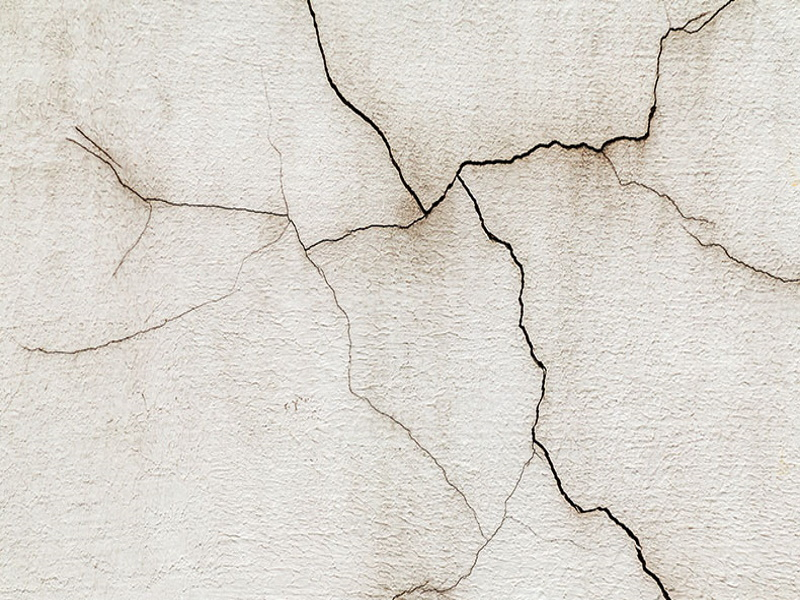
\includegraphics[width=.8\linewidth]{images/mapa_da_obra_img_fissura.jpg}
          % \caption{A subfigure}
          \label{fig:fissura01}
          \fdireta{fig:fissura01}
        \end{subfigure}%
        \begin{subfigure}{.5\textwidth}
          \centering
          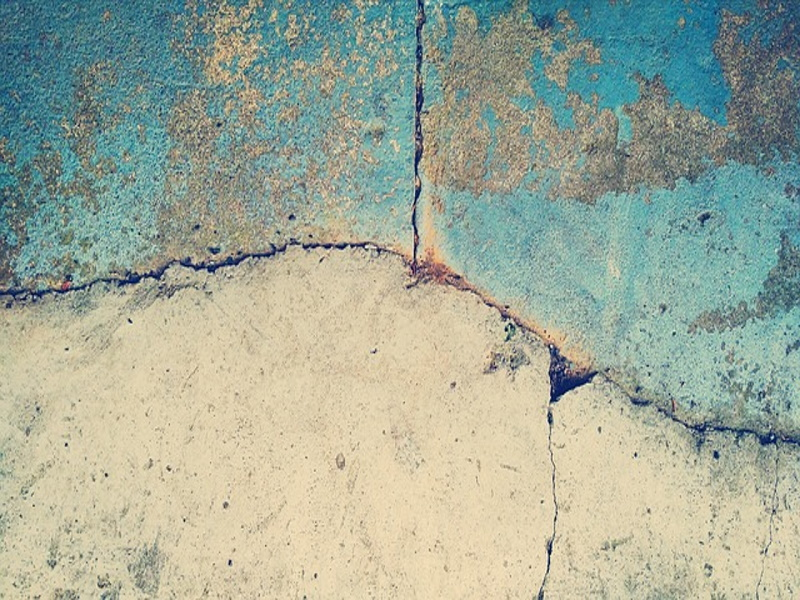
\includegraphics[width=.8\linewidth]{images/tudo_construcao_fissura02.jpg}
          % \caption{A subfigure}
          \label{fig:fissura02}
          \fdireta{fig:fissura02}
        \end{subfigure}
    
    \caption{Exemplos de fissuras em estruturas de concreto.}
    \label{fig:fissuras}
    \end{figure}

    
    \item[Corrosão de armadura:]
    
    O concreto armado consegue ser um ótimo material estrutural por conta que uma material consegue remediar os problemas de seus componentes, por exemplo, o concreto tem uma forte alcalinidade, protegendo a armadura contra corrosão \cite{pinheiro2010estruturas}.
    Porém, uma possível patologia, que geralmente acontece pela falha durante a concretagem, ou por erros de \WANDER{cálculo} para determinar a espessura do concreto, podem resultar na exposição da armadura, fazendo com que a exposição ao dióxido de carbono do ambiente faça a corrosão acontecer \cite{statera}. 
    No caso de certas OAE`s, como pontes, existem uma maior quantidade de agentes agressivos, como em zonas marítimas onde há o vento que carrega partículas de sal\cite{statera}.

    Além de ser a patologia mais usual nas estruturas de concreto armado, a corrosão de armadura também é uma das mais perigosos, sendo considerado uma anomalia grave cujo o eventual produto pode vir a ser o colapso total da estrutura\cite{tecnosil_2017}. 
    Posterior ao inicio dessa patologia, se não houver tratamento e manutenção, a corrosão manifesta uma progressão constante e ininterrupta em todos os casos \cite{tecnosil_2017}.
    
    \item[Falhas de Concretagem:]
    
    As falhas de concretagem denominam as irregularidades que ocorrem no período do processo de concretagem por conta de erros de colocação ou compactação do concreto \cite{statera}.
    Segundo SILVA(2011), projetos deficientes, de execução mal feitas são os principais responsáveis pelo surgimento de patologias.
    
    Para reprimir que tais erros ocorram, há uma série de diretrizes que cada projeto deve executar, no caso de OAE`s o órgão emissor dessas diretrizes é o DNIT. 
    Contudo, segundo \citeonline{tecnhe_2010}, no contexto atual da construção civil, não estão sendo mais seguidos os prazos sugeridos para cada etapa construtiva, diminuir o tempo de cada etapa resulta também em menos tempo para planejar e projetar as características da obra e de seus componentes.

    
\end{description}


\section{Problemas/prejuízos causados pelas fissuras}

% Repetitivo?
Embora não apresente problemas sérios diretamente, as fissuras representam o sinal inicial de que um problema sério pode vir a acontecer \cite{alani2014integrated}, por conta disso o DNIT exige que aconteça regularmente uma inspeção \cite{dnit2004}.
Uma inspeção realizada da forma correta consegue produzir várias informações do estado atual da estrutura através da
medição de grandezas físicas, como acelerações, deformações, e/ou deslocamentos.

O problema que o método tradicional de inspeção, que é o manual, pode ser considerado um trabalho extensivo, custoso, e possivelmente perigoso, além de necessitar da contratação técnicos capacitados e de confiança \cite{adhikari2014image}.
Outro grande custo é o carecimento de certas ferramentas e equipamentos, em especial em lugares de difícil acesso onde há a utilização de certos veículos especializados, como caminhão com cesta elevatório \cite{dorafshan2018bridge}.
Há ainda o fator do descontentamento gerado ao publico, pois geralmente há a necessidade de no mínimo limitar o acesso à OAE, o que também causa custos de forma indireta \cite{catbas2018vision}.

\section{Enfoque computacional para solucionar o problema}

Para solucionar tal problema, diversos autores buscam desenvolver novas ferramentas e técnicas para auxiliar o serviço de manutenção e monitoramento. 
Tais autores concordam que as melhores soluções possíveis estão dentro do campo computacional e portanto se faz necessário o estudo com enfoque computacional dentro da engenharia.

\subsection{Sensoriamento}

Uma das primeiras soluções encontradas foi a de utilizar cadeias de sensores que extrairiam dados da ponte em tempo real, para que o técnico responsável tivesse acesso a tais informações sempre que requerido \cite{spencer2019advances}.
Embora para época tenha sido uma alternativa recomendável, mesmo com as evoluções tecnologias, até hoje esta é uma solução problemática por conta dos custos exorbitantes \cite{Zhuang2022}.
Entre os desafios enfrentados se destacam: realizar a instalação da fiação de cabos por toda a estrutura, transmissão e geração de energia para sustentar a cadeia de sensores, transferência de dados entre si e para um sistema receptor, calibração regular dos sensores \cite{catbas2018vision}.

% Apresentando apenas os problemas
% Aprofundar sobre os sensores?

\subsection{Visão computacional}

Com o passar do tempo, as técnicas baseadas em visão computacional ganharam maior autoridade por conta de seus resultados em identificação, classificação e localização de objetos dentro de imagens, por conta disso \citeonline{webb2015categories} apresenta a visão como uma possibilidade para ser utilizada na engenharia civil, em especifico no âmbito da engenharia civil, e do campo de inspeções e monitoramento.

Ao utilizar imagens e vídeos como dados de analise para o computador é possível obter as informações necessárias para o monitoramento \cite{spencer2019advances} sema a necessidade do contato direto humano, evidentemente, sendo essa sua maior vantagem \cite{catbas2018vision}.

Uma outra vantagem da visão computacional é que a estratégia para captura de tais imagens e vídeos não é fixa ou precisa de um equipamento específico, imagens de alta qualidade podem ser registradas até mesmo de câmeras de telefones, mas caso se tenha um maior investimento é possível utilizar câmeras de alta performance podendo ser fixas ou móveis, entretanto, uma tecnologia que vem conquistando espaço são os \sigla{UASs}{Unmanned Aerial Systems}, mais conhecido como drones \cite{dorafshan2018bridge}. Atualmente, os drones tem conquistado espaço em vários ambientes profissionais, sendo considerado uma ferramenta eficiente, contribuitiva e uma alta relação de custo-benefício \cite{zoubir2021crack}. 
Dessa forma sendo uma ótima alternativa dentro do campo das inspeções e monitorações. 

Com essas tecnologias de visão computacional citadas e um investimento mínimo, é possível até mesmo implementar um sistema automatizado de coleta das imagens. Entretanto, mesmo com a automatização da captura de imagens, seja através de câmeras estacionarias, drones ou outro método, ainda há a parte mais tediosa e custosa em questão de tempo, que é a de um técnico especialista realizar a analise interpretativa dos dados coletado \cite{zoubir2021crack}, essa etapa porém pode ser também automatizada a partir de métodos computacionais.

\subsection{Utilização de heuristicas}

Durante o começo das pesquisas de visão computacional, as principais ferramentas a serem utilizadas para detectar problemas em estruturas eram caracterizadas como heurísticas, normalmente esses métodos eram executados utilizando com a aplicação de limiar ou com a criação de filtros específicos \cite{spencer2019advances}, que posteriormente poderiam até ser calculados utilizando aprendizagem de máquina.

Os tipos de filtros mais comuns utilizados que é utilizado até em trabalhos mais recentes são os detectores de bordas, onde a a partir de alguma premissa especificada pelo usuário um algoritmo busca em uma imagem uma série de pontos onde existam mudanças bruscas que interligados configure algum objeto, dessa forma realizando uma segmentação da imagem \cite{ziou1998edge}.

Em um dos primeiros trabalhos específicos da área, \citeonline{abdel2003analysis} utiliza os detectores de borda \textit{Sobel} e \textit{Canny} e as equações transformadas de \textit{Fourier} e \textit{Fast Haar} como gradiente para detecção de borda em 50 fotos adquiridas a partir de câmeras fotográficas e conseguindo uma acurácia dividida entre 86 e 64\% dentre seus métodos, sendo a transformada de \textit{Fast Haar} a que gerou o melhor resultado, porém sendo ainda necessário a interpretação de um usuário para separar o que realmente são fissuras dos erros causados pela textura. 

Já o autor \citeonline{jahanshahi2009survey} compara o método de detecção de borda com a união de certas técnicas morfológicas:

O processo de detecção de bordas é detalhado sobre os cálculos utilizados, sendo utilizados cálculos de derivadas de altovalores e altovetores, gradientes, filtro Gaussiano e Laplaciano, transformadas de \textit{Fast Haar}, limiarização baseada em mediana e uma pequena camada de rede neural de uma camada para caracterizar os objetos gerados, com isso obtendo uma acurácia de 71.5\%, que o próprio autor compara com último trabalho citado, de \cite{abdel2003analysis}, pela similaridade, e explica que a diferença de resultado acontece principalmente pela mudança da direção da luz conforme o tempo do dia. 

O outro método, consiste em tratar a imagem a partir de sua morfologia matemática, ou seja, uma matriz de valores da escala de cinza, os processos morfológicos mais básicos são a dilatação e erosão, a partir da combinação sendo possível realizar os processos de abertura, fechamento, gradiente morfológico, operações \textit{bottom-hat} e \textit{top-hat}, o problema é que esses processos morfológicos necessitam um elemento estruturante de tamanho apropriado para cada tipo de imagem, o que o torna menos dinâmico. Embora o autor não informe a porcentagem de acurácia, ele define esse tipo de abordagem mais efetivo que o detector de bordas pois gera menos ruido que tal.

Para finalizar, o autor \citeonline{dorafshan2019benchmarking} compara a eficiência, precisão e tempo computacional de quatro diferentes filtros aplicados junto à detecção de bordas nos domínios espacial e dois filtros aplicados no domínio de frequência. Como base de dados foi utilizado 50 imagens de concreto saudável e 50 imagens de concreto com presença de fissuras, ambos coletados através de drones. 

O método aplicado consiste em inicialmente converter a imagem para níveis de cinza dando um peso muito maior à cor verde, um valor médio ao vermelho e baixo ao azul. % Coloco a porcentagem?
A partir disso, nessa nova imagem é aplicado o filtro desejado: \textit{Roberts}, \textit{Prewitt}, \textit{Sobel} e \textit{Laplacian of Gaussian} para o domínio espacial e \textit{Butterworth} e \textit{Gaussian} para o dominio de frequência, cada filtro consiste em uma pequena matriz de valores que são utilizados a partir da operação de convolução.
Para o domínio da frequência, é necessário realizar uma transformação do domínio espacial para frequência, que é feito através da transformada de \textit{Fast Fourier}. Após a aplicação de cada filtro, é realizado um aprimoramento na imagem resultante, principalmente normalização a partir da média e desvio padrão, e correção de claridade para aumentar a visibilidade das bordas. Para finalizar é realizado a segmentação da imagem, onde resultará em uma nova imagem com o formato binário onde será positivo os locais que apresenta as rachaduras, essa conversão é realizada com um corte a partir de um limiar encontrado pelo método de \textit{Otsu}.

Para avaliar os resultados, um inspetor revisou as imagens para verificar as imagens e classifica-las de forma a ter 100 \% de acurácia em suas rotulações, logo, foi comparado os resultados dos filtros com o resultado apresentado pelo inspetor, tendo resultado entre 77\% à 92\% de acurácia, 82\% à 88\% de precisão e variação de tempo entre 1.18 e 1.92 segundos, sendo que \textit{Laplacian of Gaussian} foi o filtro com os melhores resultados, com 92\% de acurácia, 88\% de precisão e 1.18 segundos.

\wander{LUCAS EU GOSTEI DESSA PARTE SUA DAS HEURTISTICAS MAS EU RETIRARIA O TITULO DESSA SEÇÃO COMO HEURISTICAS...EU COMPREENDO HEURISTICAS DE OUTRA FORMA...NORMALMENTE AS HEURISTICAS SÃO OS PROBLEMAS DE OTIMIZAÇÃO IGUAL VC FEZ NA SUA IC...ENTÃO VEJA COM A PROFA. NUBIA MAIS EU RETIRARIA SOMENTE ESTE TÍTULO. AI LOGICAMENTE AQUELA PARTE INICIAL QUE VC DEFINIFE DE HEURISTICAS SAI.}

\wander{AQUI EU ACHO QUE NÃO PRECISA DESSA SEÇÃO...ACHO QUE VOCÊ JÁ FAZ O ESTUDO DELA NO ITEM 3 MESMO ENTÃO NÃO PRECISA COLOCAR.}
\subsection{Deep learning}

